133. \begin{figure}[ht!]
\center{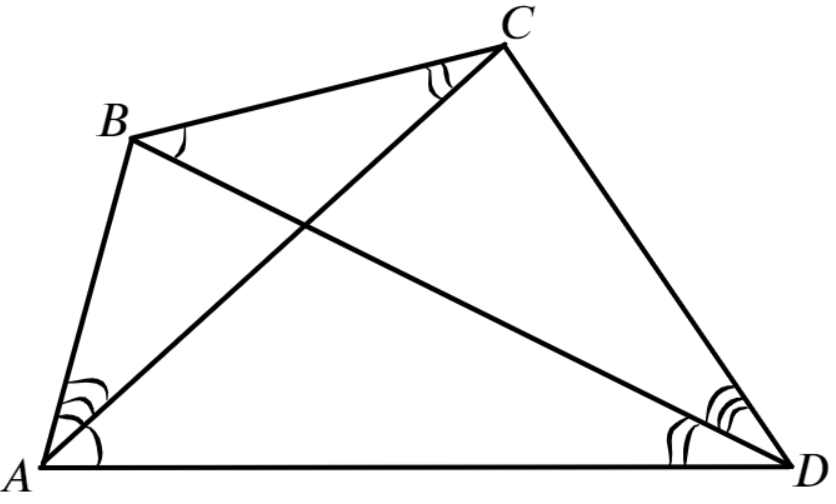
\includegraphics[scale=0.35]{g9-133.png}}
\end{figure}\\
Так как угол, образованный стороной $BC$ и диагональю $BD$ равен углу, образованному противоположной стороной $AD$ и другой диагональю $AC,$ четырёхугольник $ABCD$ является вписанным. Тогда аналогично $\angle BAC=\angle BDC,\ \angle BCA=\angle BDA,\ \angle D=\angle BDC+\angle BDA=42^\circ+37^\circ=79^\circ.$\\
